% Based on operation intensity in Section~\ref{sec:workload}, we plot the workloads in the roofline model Figure~\ref{fig:roofline}. All kernels are bounded by memory in GH200, and most of the kernels are bounded by memory in A100. 

% We further separate the situation into: fully overlapped, and fully un-overlapped. 


\section{Theoretical Analysis}\label{sec:theory}
Based on the operational intensity analysis from Section~\ref{sec:workload}, Figure~\ref{fig:roofline} shows all studied kernels are memory-bound on GH200, and most memory-bound on A100. To simplify the following discussion, we assume that all kernels are throughput-bound. 

%We consider two scenarios: latency bound and throughput bound. 
%Then we analyze two extreme cases: fully overlapped and fully un-overlapped for memory access and computation.
% \subsection{Latency-Bound}
% % \todo{Test Latency of Tensor Core}
% We simplify the discussion by comparing the latency of double precision (FP64) ptx instruction. In A100, previous research shows DMMA latency is 16 cycle~\cite{9926299}, while FP64 latency is 6 cycle~\cite{10740811}. As such, in the latency-bound scenario, the tensor core shows no advantage over the CUDA core. 

% \subsection{Throughput-Bound}

when it is throughput bound, which is usually the case in High-Performance workloads, we have time for computation $T_{\text{cmp}}=\tfrac{\mathbb{W}}{P}$. 
% \begin{equation}\footnotesize
    % T_{\text{cmp}}=\tfrac{\mathbb{W}}{P}
% \end{equation}
and time for memory access $T_{mem}=\tfrac{\mathbb{Q}}{B}$.
% \begin{equation}\footnotesize
%     T_{mem}=\tfrac{\mathbb{Q}}{B}
% \end{equation}
So we have:
\begin{equation}\footnotesize
    % T_{mem}=\tfrac{\mathbb{Q}}{B}
    \tfrac{T_{mem}}{T_{cmp}}=\tfrac{\tfrac{\mathbb{Q}}{B}}{\tfrac{\mathbb{W}}{P}}=\tfrac{\mathbb{B}}{\mathbb{I}}
\end{equation}

For memory-bound kernel, $\mathbb{B}>\mathbb{I}$, we have:
\begin{equation}\footnotesize
T_{\text{mem}} > T_{\text{cmp}}
\end{equation}

We analyze two extreme cases: fully overlapped and fully un-overlapped for memory access and computation.

\subsection{Fully Overlapped}\label{sec:anaovl}
\begin{figure}[t!]
% \vspace{-15pt}
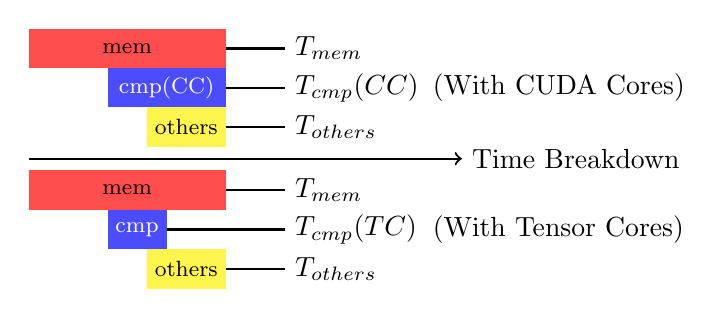
\begin{tikzpicture}[scale=0.5, every node/.style={scale=1}]
    % Timeline axis
    \draw[->, thick] (0,0) -- (11,0) node[right] {\textbf\footnotesize{Time Breakdown}};
    % Memory and Compute bars
    \fill[red!70] (0,2.3) rectangle (5,3.3) node[pos=.5,black] {\footnotesize{mem}};
    \fill[blue!70] (2,1.3) rectangle (5,2.3) node[pos=.5,white] {\footnotesize{cmp(CC)}};
    \fill[yellow!70] (3,0.3) rectangle (5,1.3) node[pos=.5,black] {\footnotesize{others}};

    \draw[thick] (5,2.8) -- (6.5,2.8) node[right] {$T_{\text{mem}}$};
    \draw[thick] (5,1.8) -- (6.5,1.8) node[right] {$T_{\text{cmp}}(CC)$};
    \draw[thick] (5,0.8) -- (6.5,0.8) node[right] {$T_{\text{others}}$};

    \draw[thick] (10,1.8) -- (10,1.8) node[right] {(With CUDA Cores)};

    \fill[red!70] (0,-0.3) rectangle (5,-1.3) node[pos=.5,black] {\footnotesize{mem}};
    \fill[blue!70] (2,-1.3) rectangle (3.5,-2.3) node[pos=.5,white] {\footnotesize{cmp}};
    \fill[yellow!70] (3,-2.3) rectangle (5,-3.3) node[pos=.5,black] {\footnotesize{others}};
    
    \draw[thick] (5,-0.8) -- (6.5,-0.8) node[right] {$T_{\text{mem}}$};
    \draw[thick] (3.5,-1.8) -- (6.5,-1.8) node[right] {$T_{\text{cmp}}(TC)$};
    \draw[thick] (5,-2.8) -- (6.5,-2.8) node[right] {$T_{\text{others}}$}; 

    \draw[thick] (10,-1.8) -- (10,-1.8) node[right] {(With Tensor Cores)};
\end{tikzpicture}
\vspace{-5pt}
\caption{Fully overlapped kernel time breakdown}\label{fig:breakout_overlap}
\end{figure}

An example of an overlapped kernel time breakdown is shown in Figure~\ref{fig:breakout_overlap}. For memory-bound kernels:
\begin{equation}\footnotesize
T = \max(T_{\text{cmp}},T_{\text{mem}},T_{\text{others}})=\max(T_{\text{mem}},T_{\text{others}})
\end{equation}
where $T_{\text{mem}}$, $T_{\text{cmp}}$, $T_{\text{others}}$ and $T$ represent memory access, computation, other operation and total times, respectively. In this scenario, reducing computation time cannot influence total runtime.

% An example of Overlapped Kernel time breakdown is shown in Figure~\ref{fig:breakout_overlap}. 
% As we are focusing on memory-bound kernel, we have:
% \begin{equation}\footnotesize
    % T_{\text{mem}} > T_{\text{cmp}}
% \end{equation}
% \begin{equation}\footnotesize
%     T = \max(T_{\text{cmp}}+T_{\text{mem}}+T_{\text{others}})=T_{mem}
% \end{equation}
% Where $T_{\text{mem}}$ is the runtime for memory access, $T_{\text{cmp}}$ is the runtime for computation, $T_{\text{others}}$ is the runtime for operations other than memory and computation, and $T$ is the total runtime. 

% In this situation, no matter how we red/uce computation, the total runtime would not change. 


\subsection{Fully Un-overlapped}\label{sec:anaunovl}
\begin{figure}[t!]
\vspace{-10pt}
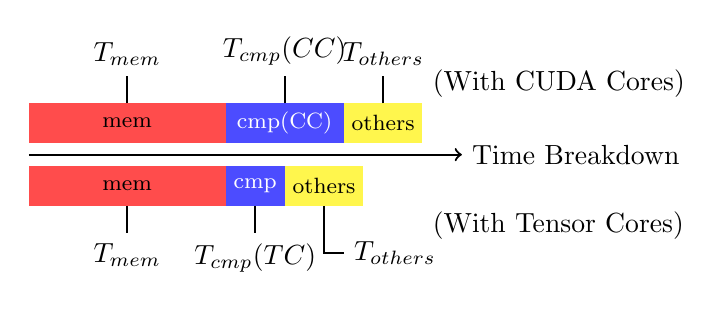
\begin{tikzpicture}[scale=0.5, every node/.style={scale=1}]
    % Timeline axis
    \draw[->, thick] (0,0) -- (11,0) node[right] {\textbf\footnotesize{Time Breakdown}};
    % Memory and Compute bars
    \fill[red!70] (0,0.3) rectangle (5,1.3) node[pos=.5,black] {\footnotesize{mem}};
    \fill[blue!70] (5,0.3) rectangle (8,1.3) node[pos=.5,white] {\footnotesize{cmp(CC)}};
    \fill[yellow!70] (8,0.3) rectangle (10,1.3) node[pos=.5,black] {\footnotesize{others}};

    \draw[thick] (2.5,1.3) -- (2.5,2) node[above] {$T_{\text{mem}}$};
    \draw[thick] (6.5,1.3) -- (6.5,2) node[above] {$T_{\text{cmp}}(CC)$};
    \draw[thick] (9,1.3) -- (9,2) node[above] {$T_{\text{others}}$};

    \draw[thick] (10,1.8) -- (10,1.8) node[right] {(With CUDA Cores)};


    \fill[red!70] (0,-0.3) rectangle (5,-1.3) node[pos=.5,black] {\footnotesize{mem}};
    \fill[blue!70] (5,-0.3) rectangle (6.5,-1.3) node[pos=.5,white] {\footnotesize{cmp}};
    \fill[yellow!70] (6.5,-0.3) rectangle (8.5,-1.3) node[pos=.5,black] {\footnotesize{others}};
    \draw[thick] (2.5,-1.3) -- (2.5,-2) node[below] {$T_{\text{mem}}$};
    \draw[thick] (5.75,-1.3) -- (5.75,-2) node[below] {$T_{\text{cmp}}(TC)$};
    \draw[thick] (7.5,-1.3) -- (7.5,-2.5) -- (8,-2.5) node[right] {$T_{\text{others}}$}; 

    \draw[thick] (10,-1.8) -- (10,-1.8) node[right] {(With Tensor Cores)};
\end{tikzpicture}
\vspace{-5pt}
\caption{Fully un-overlapped kernel time breakdown}\label{fig:breakout}
\end{figure}


For fully un-overlapped kernels (Figure~\ref{fig:breakout}):
\begin{equation}\footnotesize
T = T_{\text{cmp}}+T_{\text{mem}}+T_{\text{others}}
\end{equation}

With tensor cores providing speedup $\alpha$ ($\alpha=\tfrac{P(TC)}{P(CC)}$,$\alpha>1$): $T'_{\text{cmp}}(TC)=\tfrac{1}{\alpha}T_{\text{cmp}}(CC)$, yielding:
\begin{align}\footnotesize
Speedup&=\tfrac{T(CC)}{T(TC)} = \tfrac{T_{\text{cmp}(CC)}+T_{\text{mem}}+T_{\text{others}}}{\tfrac{1}{\alpha}T_{\text{cmp}(CC)}+T_{\text{mem}}+T_{\text{others}}} \\
&=1+\tfrac{{\alpha}-1}{1+{\alpha}\tfrac{T_{\text{mem}}+T_{\text{others}}}{T_{\text{cmp}}(CC)}} 
\\
&=1+\tfrac{{\alpha}-1}{1+{\alpha}\tfrac{T_{\text{cmp}}(CC)\times\tfrac{\mathbb{B}}{\mathbb{I}}+T_{\text{others}}}{T_{\text{cmp}}(CC)}} \\
&<1+\tfrac{\alpha-1}{1+\alpha(\tfrac{\mathbb{B}}{\mathbb{I}})}
\end{align}
% \begin{align}\footnotesize
% Speedup&=1+\tfrac{{\alpha}-1}{1+{\alpha}\tfrac{T_{\text{cmp}}(CC)\tfrac{\mathbb{B}}{\mathbb{I}}+T_{\text{others}}}{T_{\text{cmp}}(CC)}} \
% &<1+\tfrac{\alpha-1}{1+\alpha(\tfrac{\mathbb{B}}{\mathbb{I}})}
% \end{align}
% \subsubsection{}

% \noindent\textbf{Tensor Core Upper Bound:} we assume that $\alpha\to\infty$:
% \begin{align}\footnotesize
% Speedup <1+\tfrac{\mathbb{I}}{\mathbb{B}}
% \end{align}
% Example: $Speedup_{A100}(\text{GEMV})<1.05$x

\noindent\textbf{Tensor Core Upper Bound:} For memory-bound kernel, we have $T_{\text{cmp}}\to T_{\text{mem}}$:
\begin{align}\footnotesize
Speedup<1+\tfrac{\alpha-1}{1+\alpha}=2-\tfrac{2}{1+\alpha}
\end{align}
Example: FP64 Nvidia GPUs (with $\alpha=2$): $Speedup<1.33$.

\noindent Example: Assuming that $\alpha\to\infty$, we have $Speedup<2$.

\noindent\textbf{Workload Upper Bound:} we assume that $\alpha\to\infty$:
\begin{align}\footnotesize
Speedup <1+\tfrac{\mathbb{I}}{\mathbb{B}}
\end{align}
Example: $Speedup_{A100}(\text{GEMV})<1.05$.

% For memory throughput-bound workloads:
% \begin{equation}
% T_{\text{cmp}}=\tfrac{\mathbb{W}}{P}, \quad T_{\text{mem}}=\tfrac{\mathbb{Q}}{B}
% \end{equation}
% Therefore:
% \begin{equation}
% \tfrac{T_{\text{mem}}}{T_{\text{cmp}}}=\tfrac{\tfrac{\mathbb{Q}}{B}}{\tfrac{\mathbb{W}}{P}}=\tfrac{\mathbb{B}}{\mathbb{I}}
% \end{equation}
% From Equation~\ref{eqt:spup_0}:
% \begin{align}\footnotesize
% Speedup&=1+\tfrac{{\alpha}-1}{1+{\alpha}\tfrac{T_{\text{cmp}}(CC)\tfrac{\mathbb{B}}{\mathbb{I}}+T_{\text{others}}}{T_{\text{cmp}}(CC)}} \
% &<1+\tfrac{\alpha-1}{1+\alpha(\tfrac{\mathbb{B}}{\mathbb{I}})}
% \end{align}




% Additionally, when it is throughput bound, which is usually the case in High Performance workloads, we have: 
% \begin{equation}
%     T_{\text{cmp}}=\tfrac{\mathbb{W}}{P}
% \end{equation}
% And
% \begin{equation}
%     T_{mem}=\tfrac{\mathbb{Q}}{B}
% \end{equation}
% So we have:
% \begin{equation}
%     % T_{mem}=\tfrac{\mathbb{Q}}{B}
%     \tfrac{T_{mem}}{T_{cmp}}=\tfrac{\tfrac{\mathbb{Q}}{B}}{\tfrac{\mathbb{W}}{P}}=\tfrac{\mathbb{B}}{\mathbb{I}}
% \end{equation}
% So we have:
% \begin{align}\footnotesize
%     Speedup&=\tfrac{T(CC)}{T(TC)} = 
%              =1+\tfrac{{\alpha}-1}{1+{\alpha}\tfrac{T_{mem}+T_{others}}{T_{cmp}(CC)}} \\
%              &=1+\tfrac{{\alpha}-1}{1+{\alpha}\tfrac{T_{cmp}(CC)*\tfrac{\mathbb{B}}{\mathbb{I}}+T_{others}}{T_{cmp}(CC)}} 
% \end{align}
% Since ${T_{other}}>0$, we have:
% \begin{align}\footnotesize
%     Speedup &<1+\tfrac{\alpha-1}{1+\alpha*(\tfrac{\mathbb{B}}{\mathbb{I}})}
% \end{align}


% Here if we assume that $\alpha=\infty$, we have:
% \begin{align}\footnotesize
%     Speedup <1+\tfrac{\mathbb{I}}{\mathbb{B}}
% \end{align}

% We analyzed the situation of the fully overlapped and fully un-overlapped situation of memory-bound kernels. However, in real-world situations, the kernel might be partially overlapped or partially overlapped, which means the speedup would range from $1$x to $1.33$x. Further speedup would require memory access optimization, which is not exclusive to the tensor core. Data would is loaded to register file before going to tensor core or cuda core either way. 

\subsection{Summary}


Our analysis covers the two extremes of memory-computation overlap. Real-world kernels typically exhibit partial overlap, resulting in speedups between 1× and 1.33× for double precision. Performance differences beyond that would require memory access optimizations, which, we argue, function equally when applied to tensor and CUDA cores since both access data through the register file (As Figure~\ref{fig:tcarch} shows).

% The implication of the analysis in this section is that simply applying tensor core on the double precision memory-bound kernel can not get any speedup or get at most $1.33$x speedup. 

%Further speedup implies that memory access is also optimized to some extent. However, as the current Nvidia GPU memory hierarchy (Figure~\ref{fig:tcarch}) implies, the memory access optimizations are not exclusive to the tensor core. 

% \subsection{Summarize}
